\chapter{Background}\label{chap:background}

The following part is to provide a short introduction into the theory of reinforcement learning, the Soft Actor Critic Algorithm (SAC) as well to Variational Autoencoders (VAE) and Conditional Variational Autoencoders (CVAE).
\todo{update!!!}



\section{RL Framework}\label{sec:RL-Framework}

Learning is a topic that is present in all our lives since their beginning. We all learn to move our arms, like an infant that is wiggling around, learn to walk, to speak and more or less any other skill that we find in our personal repository until now.  

Reinforcement Learning (RL) is about to have a computational approach to this kind of learning.
In the class of RL-Problems the environment provides a challenge like, riding a bicycle. But it is not told how this goal can be achieved.  Therefore it has be learned how to derive actions from situations on or off the bike in order to complete this task or - speaking of the numerical approach - maximize a reward function.
In most cases the problem solving methods that are classified as RL-methods are applied on tasks that require not only a sequence of actions to interact with an environment but also some kind of feedback.
Therefore these setups are designed to provide this kind of feedback. Either if it is an immediate feedback like an additional time step the agent has not crashed the bike or if it is more like a long shot feedback, for example a bonus that the agent has earned after a board game. 
These principals can be boiled down to three main characteristics of reinforcement learning problems:

\begin{itemize}
    \item There is a closed loop mechanism between actions and feedback that is provided by the environment where the agent is operating in.
    \item The agent is not given any direct instructions how to solve the given problem.
    \item The actions an agent is performing have consequences over time. Either for him or the environment he is working in.  
\end{itemize}

Before we can have an exemplary look on the closed loop mechanics, we would like to introduce a couple of key components of RL including the Markov Decision Process.

Every agent exists in a specified environment and also interacts within a sequence of discrete time steps $t \in \mathbb{N}$. In order to do so the agent has to perceive the environment through a \textbf{state} representation $S_t \in \mathcal{S}$ which is an element of all possible states, the state space $\mathcal{S}$. To really interact with the environment the agent has to perform an \textbf{action} $A_t \in \mathcal{A}(S_t)$ where $\mathcal{A}(S_t)$ is the set of all possible actions in given state $S_t$. To chose an action the agent calculates for each possible action $A_t$ a probability $\pi_t(A_t|S_t)$ for a given state $S_t$ and chooses the maximum with respect to the given actions. To achieve a more compact notation we will refer to the action $A_t = a$, the state $S_t = s$ and therefore also the policy as $\pi_t(a|s)$.  
This probability distribution is called the \textbf{policy}. 
After the agent has chosen and executed an action, which also mean we will move one time step further $t \to t + 1$, the environment will return the next state $S_{t+1}$ the agent will perceive and a \textbf{reward} $R_{t+1} \in \mathbb{R}$.\\
The long term goal of the agent is to adapt its policy to maximize the total amount reward the agent receives from the environment.

\begin{figure}[htb!]
	\centering
	\minipage{0.5\textwidth}
    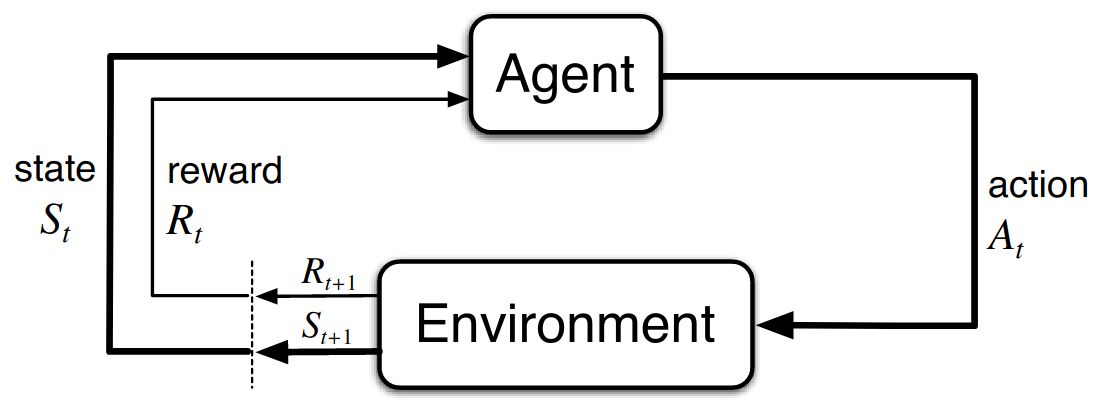
\includegraphics[width=\linewidth,]{figures/background/agent-environment-interaction.png}
	\caption{interaction between agent and the environment}
	\label{fig:agent-environment_interaction}
	\endminipage
\end{figure}
\todo{cite figure}


\todo{
Explain the concept of reinforcement learning and its applications
Describe the Markov decision process (MDP) and the Bellman equation
Discuss the challenges of using reinforcement learning in practice}

\section{Soft Actor Critic}
Briefly explain what the SAC algorithm is and why it is important
Provide a preview of what the chapter will cover

L1 smooth loss for $x, y \in \mathbb{R}$
\begin{equation}
    \mathcal{L}_\beta(x_i, y_i) = \begin{cases} \frac{1}{2 \beta} \cdot (x_i - y_i)^2 & \text{if $|x_i - y_i| < \beta$} \\ |x_i - y_i| -  \frac{\beta}{2} & \text{else}\end{cases} \\ 
\end{equation}

\subsection{Actor-Critic Algorithms}

% Describe the basic actor-critic architecture and its limitations
% Explain the difference between on-policy and off-policy learning
% Describe the advantage of using a critic in the actor-critic algorithm
The basic actor-critic architecture is a type of reinforcement learning algorithm that consists of two components: an actor and a critic. The actor is responsible for selecting actions based on the current state, while the critic evaluates the quality of the actor's actions by estimating the expected return from the current state. The actor uses this feedback from the critic to adjust its policy and improve its performance.

On-policy learning and off-policy learning refer to different methods for updating the policy in reinforcement learning. In on-policy learning, the agent learns from the data generated by its current policy, while in off-policy learning, the agent learns from data generated by a different policy. On-policy learning can be more stable, but it may require more data to converge. Off-policy learning can be more efficient, but it can be more sensitive to the quality of the data.

The advantage of using a critic in the actor-critic algorithm is that it provides a more stable feedback signal than using only rewards. The critic estimates the expected return from a state, which takes into account the long-term consequences of actions. This allows the actor to learn from the critic's feedback and improve its performance more efficiently than if it only received reward signals. Additionally, the critic can help to generalize across different states and actions, improving the overall performance of the algorithm.

One limitation of the basic actor-critic architecture is that it can suffer from high variance and slow convergence due to the interaction between the actor and critic. This can be addressed through the use of techniques such as baseline subtraction and eligibility traces.

\subsection{Soft Actor Critic Algorithm}
% Explain the concept of entropy regularization and its role in the SAC algorithm
% Describe the architecture of the SAC algorithm and how it differs from traditional actor-critic algorithms
% Explain how the actor and critic are trained using the maximum entropy objective
% Discuss the advantages of the SAC algorithm, such as improved sample efficiency and exploration


\begin{algorithm}
\caption{Soft Actor Critic}\label{alg:SAC}
\begin{algorithmic}
    \State{} Input: initial policy parameters $\theta$, Q-function parameters $\phi_0$, $\phi_1$, empty replay buffer $\mathcal{D}$
        \State{} Set target parameters equal to main parameters $\phi_{\text{target}, 0}$ $\leftarrow$ $\phi_0$, $\phi_{\text{target}, 1}$ $\leftarrow$ $\phi_1$ 
        \For{$i$ in number of epochs}
        \State{} $s$ $\leftarrow$ reset environment
        
        \For{$t$ number of timesteps}
        \State{} $a$ $\sim$ $\pi_\theta(\cdot | s)$
        \State{} $s'$, $r$, $d$ $\leftarrow$ execute $a$ in environment
        \State{} Store $(s, a, r, s', d)$ in replay buffer $\mathcal{D}$
        \If{$d$ is true}
        \State{} break and reset environment
        \EndIf{}
        \State{} $s$ $\leftarrow$ $s'$
        \EndFor{}
        
        \If{$|\mathcal{D}|$ > minimal buffer size}
        \For{number of train iterations}
        \State{} sample minibatch: $(s_\mathcal{B}, a_\mathcal{B}, r_\mathcal{B}, s'_\mathcal{B}, d_\mathcal{B}) = \mathcal{B}$ $\leftarrow$ $\mathcal{D}$ 
        \State{} compute td target $y$ with $\tilde{a}'_\mathcal{B} \sim \pi_\theta(\cdot|s'_\mathcal{B})$
        \begin{equation}\label{eqn:td-target-batch}
            y(r_\mathcal{B}, s'_\mathcal{B}, d_\mathcal{B}) = r + \gamma \cdot d \cdot \left(\min_{i\in\{0, 1\}}\left(Q_{\phi_{\text{target}, i}}(s'_\mathcal{B}, \tilde{a}'_\mathcal{B})\right) - \alpha \cdot \log\left(\pi_\theta(\tilde{a}'_\mathcal{B}|s'_\mathcal{B})\right)\right)
        \end{equation}
        \State{} Update Q-functions for parameters $\phi_i$ $i \in \{0, 1\}$ using:
        \begin{equation}\label{eqn:q-update}
            \nabla_{\phi_i} \frac{1}{|B|} \sum_{k \in |\mathcal{B}|}\mathcal{L}_\beta\left(y(r_{\mathcal{B}, k}, s'_{\mathcal{B}, k}, d_{\mathcal{B}, k}), Q_{\phi_i}(s_{\mathcal{B}, k}, a_{\mathcal{B}, k})\right)    
        \end{equation}
        \State{} Update policy with $\tilde{a}_\mathcal{B} \sim \pi_\theta(\cdot|s_\mathcal{B})$ using:
        \begin{equation}\label{eqn:policy-update}
           \nabla_{\theta} \frac{1}{|\mathcal{B}|}\sum_{k \in |\mathcal{B}|}\min_{i\in\{0, 1\}}Q_{\phi_i}(s_{\mathcal{B}, k}, \tilde{a}_{\mathcal{B}, k}) - \alpha \cdot \log\left(\pi_\theta(\tilde{a}_{\mathcal{B}, k}|s_{\mathcal{B}, k}\right))
        \end{equation}
        \State{} Update $\alpha$ with target entropy $H_\text{target}$ and $\tilde{a}_\mathcal{B} \sim \pi_\theta(\cdot|s_\mathcal{B})$ using:
        \begin{equation*}
            \nabla_\alpha -\frac{\alpha}{|\mathcal{B}|} \sum_{k \in |\mathcal{B}|} \left(\log\left(\pi_\theta(a'_{\mathcal{B}, k}|s_{\mathcal{B}, k})\right)\ - H_\text{target}\right)
        \end{equation*}
        \State{} Update target networks $\phi_{\text{target}, i}$ $i \in \{0, 1\}$ with $\phi_i$ $i \in \{0, 1\}$ using:
        \begin{equation*}
            \phi_{\text{target}, i} \leftarrow \rho \phi_{\text{target}, i} + (1 - \rho) \phi_i
        \end{equation*}
        \EndFor{}
        \EndIf{}
        \EndFor{}
\end{algorithmic}
\end{algorithm}

\subsection{SAC in Practice}

% Provide examples of real-world applications of the SAC algorithm, such as robotics and game playing
% Explain how the SAC algorithm can be used in continuous action spaces
% Describe the limitations of the SAC algorithm and how they can be addressed

In robotics, the SAC algorithm has been used to control robots in tasks such as grasping objects, locomotion, and manipulation. The SAC algorithm's ability to handle continuous action spaces makes it a suitable choice for robotic control, where fine-grained control is often required.

In game playing, the SAC algorithm has been used to train agents to play video games such as Atari and Super Mario Bros. The SAC algorithm's ability to balance exploration and exploitation makes it effective in game playing, where agents must learn to navigate complex environments and respond to changing conditions.

The chapter also discusses how the SAC algorithm can be used in continuous action spaces. The SAC algorithm uses a Gaussian distribution to represent the policy, which allows it to handle continuous action spaces. The use of a Gaussian distribution also enables the SAC algorithm to handle multimodal policies, where multiple actions can be appropriate for a given state.

Finally, the chapter discusses the limitations of the SAC algorithm and how they can be addressed. The SAC algorithm can suffer from high variance and slow convergence, especially in high-dimensional state spaces. This can be addressed through techniques such as batch normalization, automatic entropy adjustment, and value function regularization. The chapter also discusses future directions for research, such as incorporating model-based methods into the SAC algorithm to improve sample efficiency.

Conclusion:
The Soft Actor Critic algorithm is a powerful approach to reinforcement learning that has been applied in a variety of domains, including robotics and game playing. Its ability to handle continuous action spaces makes it a suitable choice for many real-world applications. However, the SAC algorithm has limitations that must be addressed, such as high variance and slow convergence. These limitations can be addressed through the use of appropriate techniques and future research directions. The SAC algorithm is an exciting area of research with potential applications in many fields.

% \subsection{Extensions to SAC}
% 
% Describe extensions to the basic SAC algorithm, such as distributed SAC and multi-agent SAC
% Explain how SAC can be combined with other models, such as generative models

% \subsection{Current and Future Directions}
% 
% Describe current research trends in SAC, such as improving its performance in high-dimensional state spaces and addressing the issue of multi-task learning
% Discuss potential future applications of SAC, such as in healthcare and finance
% Explain challenges that must be addressed in order for SAC to continue to advance

% \subsection{Conclusion}
% 
% Summarize the main points of the chapter
% Emphasize the importance of SAC in a variety of fields
% Encourage further exploration of the topic.
 
\section{Neural Networks}

Briefly explain what neural networks are and why they are important
Provide a preview of what the chapter will cover

% \subsection{Historical Overview}
% 
% Discuss the early history of neural networks, including the work of Warren McCulloch and Walter Pitts in the 1940s
% Explain how the field evolved in the 1950s and 1960s
% Discuss the challenges faced by researchers during this time, including the limitations of computing power and the lack of effective training algorithms

\subsection{The Rise of Deep Learning}

Explain how the development of new algorithms and the availability of large datasets led to a resurgence in interest in neural networks in the 2000s
Describe the key breakthroughs that made deep learning possible, including the development of convolutional neural networks and recurrent neural networks
Provide examples of important applications of deep learning, such as image and speech recognition

\subsection{Neural Network Architecture}

% Explain the basic architecture of a neural network, including the role of input and output layers, hidden layers, and activation functions
% Describe different types of neural networks, including feedforward networks, recurrent networks, and convolutional networks
% Explain how neural networks can be trained using techniques such as backpropagation and stochastic gradient descent

Neural networks are a type of machine learning model inspired by the structure and function by the cell type of neurons. It consists like their biological paradigm, of interconnected layers of individual units, called neurons.

The basic architecture as in \figref{fig:neural_network_schema/architecture}, of a neural network includes an input layer (yellow), one or more hidden layers (blue and green), and an output layer (red). The input layer receives the input data, which is then passed through the hidden layers before producing the output. This is why we call this basic architecture a feed forward neural network. The number of nodes in each layer and the connections between them are dictated by the architecture of a network.

\begin{figure}
    \begin{center}
        \subfloat[schematic drawing of a feed forward neural network]{
            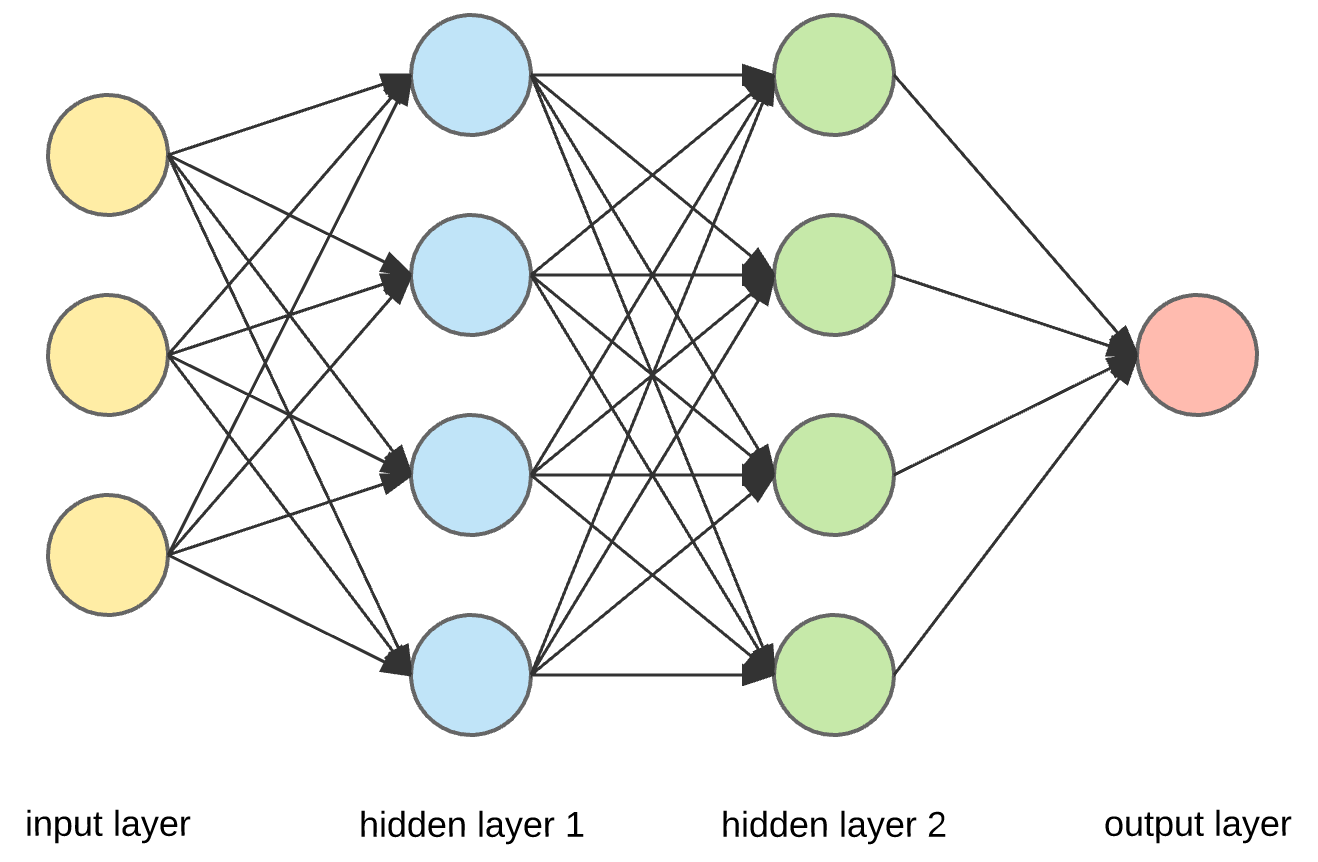
\includegraphics[width=0.4\linewidth]{figures/background/neural_network_architecture.png}
            \label{fig:neural_network_schema/feed-forward-architecture}
            }
        \hfill
        \subfloat[schematic drawing of a single neuron]{
            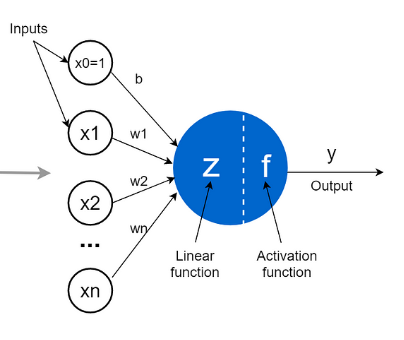
\includegraphics[width=0.4 \linewidth]{figures/background/neuron_schema.png}
            \label{fig:neural_network_schema/neuron}
            } 
    \end{center}
    \caption[neural network and neuron schema]{The figure shows the schematic drawing of a feed forward neural network and a neuron}
    \label{fig:neural_architecture}
\end{figure}

Each neuron as in \figref{fig:neural_network_schema/neuron}, is designed in the same way. First it calculates a weighted $z$ of its inputs $x$, the corresponding weights $w$ and bias $b$ before passing it on to an activation function $h$. This function is designed to introduce nonlinearity into the model, allowing it to capture complex relationships between variables otherwise the whole network would be a single linear combination of its inputs and weights. Common activation functions include the sigmoid function, the hyperbolic tangent function, and the rectified linear unit (ReLU) function as in \figref{fig:action_function}

\begin{figure}[t]
    \begin{center}
        \subfloat[Sigmoid]{
            
\includegraphics[width=0.3\linewidth]{figures/place_holder.png}
            \label{fig:activation_function/sigmoid}
            }
        \hfill
        \subfloat[hyperbolic tangent function]{
            
\includegraphics[width=0.3\linewidth]{figures/place_holder.png}
            \label{fig:activation_function/tanh}
            }
        \hfill
        \subfloat[rectified linear unit]{
            
\includegraphics[width=0.3\linewidth]{figures/place_holder.png}
            \label{fig:activation_function/relu}
            }
    \end{center}
    \caption[common activation functions in a neural network]{\textbf{common activation functions in a neural network}}
    \label{fig:action_function}
\end{figure}

There are several types of neural networks, including feedforward networks, recurrent networks, and convolutional networks. Feedforward networks are the simplest type of neural network, consisting of a series of layers that process information in a single direction. Recurrent networks, on the other hand, allow information to be passed between nodes in a cyclical manner, making them suitable for processing sequential data. Convolutional networks are designed for image processing tasks and use convolutional layers to identify patterns and features within images.

Neural networks are trained using techniques such as backpropagation and stochastic gradient descent. Backpropagation is an algorithm for calculating the gradient of the error with respect to the weights of the network, which can then be used to update the weights and improve the performance of the model. Stochastic gradient descent is a technique for minimizing the error of the model by iteratively adjusting the weights based on randomly selected subsets of the training data. These techniques allow neural networks to learn from large datasets and make accurate predictions on new data.

\subsection{Supervised Learning}

\subsection{Applications of Neural Networks}

% Provide examples of real-world applications of neural networks, such as natural language processing, computer vision, and autonomous vehicles
% Discuss the advantages and limitations of neural networks in different domains

Neural networks are widely used in real-world applications like in computer vision, marketing or medical applications. Particularly in combination with reinforcement learning they are successfully used in robotics for object recognition and manipulation, in gaming for complex decision-making, and in finance for predicting stock prices.

% \subsection{Current and Future Directions}
% 
% Describe current research trends in neural networks, such as transfer learning and % reinforcement learning
% Discuss potential future applications of neural networks, such as personalized medicine and % climate modeling
% Explain challenges that must be addressed in order for neural networks to continue to advance

% \subsection{Conclusion}
% 
% Summarize the main points of the chapter
% Emphasize the importance of neural networks in a variety of fields
% Encourage further exploration of the topic.


\section{Variational Autoencoder}
In this chapter we want to provide a intuition about Autoencoders 
Based on the manifold hypothesis

appoaches to solve this by principal component analysis
Is a technique of unsupervised learning

\subsection{Introduction}

Variational autoencoders (VAEs) and conditional variational autoencoders (CVAEs) are types of deep generative models that are used for unsupervised learning. Unsupervised learning is a type of machine learning where the model is not given labeled data for training. Instead, the model is tasked with finding patterns or structure in the data on its own. The goal of unsupervised learning is often to find hidden relationships or groupings within the data that can be used for further analysis or decision-making
VAEs and CVAEs are important because they can learn to generate realistic and diverse samples from complex high-dimensional data distributions, such as images or audio.

\subsection{Autoencoders}

% Describe traditional autoencoders and their limitations
% Explain how autoencoders can be used for unsupervised learning

Lets start with a Autoencoder. An Autoencoder $f = d \circ e$ consists of two function approximators in series, one encoder $e$ and one decoder $d$. In most cases these function approximators are resembled by neural networks.

In a forward pass through the module first the encoder maps the high dimensional input $x \in \mathbb{X}$ into a lower dimensional latent space $z \in \mathbb{Z}$, $z = e(x)$. This latent vector $z$ contains with a trained encoder, an encoding of certain properties from the input $x$. Therefor similar input values $x$ should correspond to similar latent vectors $z$. \\
In the second stage we map the latent vector $z$ back into the high dimensional features space $X$, $d: \mathbb{Z} \to \mathbb{X}$. This should optimally reconstruct the given input $\hat{x} = d(z) = d(e(x))$. \\

\begin{figure}[t]
    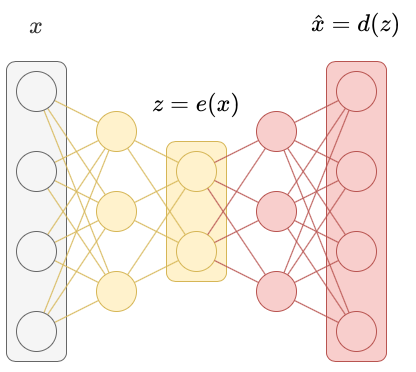
\includegraphics[width=0.5\linewidth]{figures/background/AE.png}
    \caption[Autoencoder schematics]{\textbf{schematic drawing of a Autoencoder}}
    \label{fig:Autoencoder_schematics}
\end{figure}

\subsection{Variational Autoencoders}

A VAE is very similar to a basic Autoencoder. It also contains an encoder and a decoder. The key difference lays in the in the latent variable. Instead of feeding the output from the encoder directly into the decoder the latent variable gets sampled from a parameterized distribution. The parameters for this distributions are the output from the encoder.

Explain the concept of a latent variable and how it relates to VAEs
Describe the architecture of a VAE and how it differs from a traditional autoencoder
Explain how the encoder and decoder are trained using a variational inference approach
Describe the role of the Kullback-Leibler (KL) divergence in the loss function

\subsection{Conditional Variational Autoencoders}

\begin{figure}
    \begin{center}
        
\includegraphics[width=0.5\linewidth]{figures/place_holder.png}
        \caption[Conditional Variational Autoencoder schematics]{\textbf{schematic drawing of a conditional Variational Autoencoder}}
        \label{fig:conditional-Variational_Autoencoder_schematics}
    \end{center}
\end{figure}
% Describe the architecture of a CVAE and how it differs from a VAE
% Explain how CVAEs can be used for supervised learning tasks
% Describe the role of the conditional input in the encoder and decoder
A Conditional Variational Autoencoder (CVAE) is an extension of the VAE architecture that takes into account conditional information. In a CVAE, both the encoder and decoder are modified to accept an additional input that represents the conditional information. This input is usually in the form of a label or a set of labels that describe the class or category to which the input belongs.


The architecture of a CVAE is similar to that of a VAE, with the addition of the conditional input. The encoder takes the input data and the conditional input, and maps them to a latent space representation. The decoder takes the latent space representation and the conditional input, and maps them back to the input space.

CVAEs can be used for supervised learning tasks, where the goal is to generate samples that belong to a specific category or class. In this case, the conditional input represents the class label or category to which the input data belongs. By conditioning the generation process on the class label, the CVAE can learn to generate samples that are representative of that class.

The role of the conditional input in the encoder is to help the model capture the conditional dependencies between the input data and the class label. The encoder must learn to map both the input data and the conditional input to a meaningful latent space representation that captures the relevant information for the generation process. In the decoder, the conditional input is used to guide the generation process and ensure that the generated samples are representative of the specified class.

\subsection{VAEs and CVAEs in Practice}

% Provide examples of real-world applications of VAEs and CVAEs, such as image and text generation, and conditional image generation
% Explain how VAEs and CVAEs can be used for data compression and denoising
% Describe the advantages and limitations of VAEs and CVAEs compared to other % generative models

VAEs and CVAEs have been successfully applied to a wide range of real-world applications. In image generation, VAEs have been used to generate novel images of faces, objects, and scenes. Similarly, CVAEs have been used for conditional image generation, allowing for the generation of images based on specific attributes or classes. In text generation, VAEs have been used to generate natural language sentences and paragraphs.

VAEs and CVAEs can also be used for data compression and denoising. By learning a compressed representation of the input data, VAEs and CVAEs can reduce the dimensionality of the input space while preserving important features. Similarly, by learning to reconstruct the original input from noisy or corrupted data, VAEs and CVAEs can be used for denoising and data restoration.

One of the advantages of VAEs and CVAEs is their ability to learn a continuous latent representation of the input data. This allows for easy manipulation and exploration of the latent space, enabling applications such as image editing and style transfer. Additionally, VAEs and CVAEs can be trained using stochastic gradient descent, making them computationally efficient for large datasets.

However, VAEs and CVAEs have some limitations. The generated samples may not be as sharp or detailed as those produced by other generative models such as GANs. Additionally, the trade-off between the reconstruction loss and the KL divergence term can be difficult to balance, potentially leading to overfitting or underfitting. Nonetheless, VAEs and CVAEs remain a popular and powerful tool for generative modeling and data compression.

% \subsection{Extensions to VAEs and CVAEs}
% 
% Describe extensions to the basic VAE and CVAE architectures, such as hierarchical VAEs and semi- supervised VAEs
% Explain how VAEs and CVAEs can be combined with other models, such as Generative Adversarial % Networks (GANs)

% \subsection{Current and Future Directions}
% 
% Describe current research trends in VAEs and CVAEs, such as improving the quality of generated samples and addressing the mode collapse problem
% Discuss potential future applications of VAEs and CVAEs, such as in healthcare and climate modeling
% Explain challenges that must be addressed in order for VAEs and CVAEs to continue to advance

% \subsection{Conclusion}
% 
% Summarize the main points of the chapter
% Emphasize the importance of VAEs and CVAEs in a variety of fields
% Encourage further exploration of the topic.

\section{Inverse Kinematics}

Inverse kinematics (IK) is a fundamental problem in robotics, animation or virtual reality that involves finding a required joint angle configuration or positions to reach a desired end-effector position and optionally a desired orientation. It plays a crucial role in controlling the motion and manipulation of robotic systems, enabling them to interact with the environment and perform complex tasks. 
In this section you will find a brief summary of existing approaches, a deeper explanation of the Cyclic Coordinate Descent algorithm and the description of the used inverse kinematics RL environment.

\subsection{Existing Approaches to Solve Inverse Kinematics}
\todo{subsection created by chatGPT}

Numerous approaches have been proposed to solve the inverse kinematics problem. These approaches can be broadly categorized into analytical methods, numerical methods, heuristic methods, sampling-based methods, and machine learning-based methods.

\textbf{Analytical Methods}: Some robotic systems with simple geometries and kinematic structures can be solved analytically using closed-form solutions. Analytical methods often rely on geometric techniques and mathematical equations such as the Denavit-Hartenberg (DH) parameters to derive explicit formulas for the joint angles. These methods provide fast and exact solutions when applicable, but they are limited to specific cases with well-defined geometric relationships.

\textbf{Numerical Methods}: Numerical methods for inverse kinematics aim to iteratively approximate the joint angles that satisfy the desired end-effector position and orientation. Jacobian-based methods, such as the Jacobian transpose method and the Jacobian pseudo-inverse method, leverage the Jacobian matrix to relate the end-effector velocities to the joint velocities. These methods iteratively adjust the joint angles based on the discrepancy between the actual and desired end-effector positions. Other numerical techniques, including cyclic coordinate descent, Gauss-Newton, Levenberg-Marquardt, and optimization algorithms like Particle Swarm Optimization and Genetic Algorithms, aim to find optimal joint configurations by minimizing an objective function that represents the error between the desired and actual end-effector positions.

\textbf{Heuristic Methods}: Heuristic methods, such as the Forward and Backward Reaching Inverse Kinematics (FABRIK) algorithm, iteratively propagate positions along the kinematic chain to converge on the desired end-effector position. These methods provide an intuitive and efficient way to solve inverse kinematics problems and handle complex robotic structures with multiple degrees of freedom.

\textbf{Sampling-Based Methods}: Sampling-based methods, such as Randomized Kinodynamic Planning (RRT), adopt a randomized search strategy to explore the joint space and find feasible solutions to the inverse kinematics problem. By sampling and connecting valid configurations in the joint space, these methods can discover feasible joint angles that satisfy the end-effector constraints.

\textbf{Machine Learning-based Methods}: Machine learning approaches, including neural networks and reinforcement learning algorithms, have been increasingly explored for solving inverse kinematics. Neural networks can be trained to approximate the inverse kinematics mapping based on input-output data pairs. Reinforcement learning algorithms, such as Soft Actor-Critic (SAC), can learn inverse kinematics policies through trial-and-error interactions with the environment, optimizing joint configurations to achieve desired end-effector positions.

\subsection{Cyclic Coordinate Descent}

Cyclic Coordinate Descent (CCD) is a popular numerical method for solving inverse kinematics. It is an iterative algorithm that adjusts the joint angles of a robotic system one at a time, from a base joint to the end-effector, in order to align the end-effector with the desired target position.

The algorithm works by iteratively updating the joint angles based on the discrepancy between the current and desired end-effector positions ($p_\text{target}$). At each iteration, CCD focuses on a single joint and adjusts its angle to minimize the positional error. By sequentially updating the joint angles in a cyclic manner, CCD aims to converge towards a solution that satisfies the desired end-effector position.

\begin{algorithm}
    \caption{Cyclic Coordinate Descent Pseudo Code}\label{alg:CCD}
    \begin{algorithmic}
        \State{} Input: Current joint angles $q$, Desired end-effector position $p_\text{target}$.
        \While{unitl convergence}
            \For{each $i$ in $[N-1, \ldots, 0]$}
                \State{} Calculate the vector from the current joint position to the end-effector position:
                \State{} $V_\text{current} \leftarrow p_{N-1} - p_i$

                \State{} Calculate the vector from the current joint position to the target position:
                \State{} $v_\text{target} \leftarrow p_\text{target} - p_i$

                \State{} Calculate the rotation necessary to align $v_\text{current}$ with $v_\text{target}$:
                \State{} $\delta q_i \leftarrow \text{angle\textunderscore between}(v_\text{current}, v_\text{target})$

                \State{} Update the joint angel:
                \State{} $q_i \leftarrow q_i + \delta q_i$
            \EndFor{}
        \EndWhile{}
\end{algorithmic}
\end{algorithm}

As illustrated in \algoref{alg:CCD} and \figref{fig:background/CCD geometry} in each iteration, CCD calculates the vector from the current joint position $p_i$ with $p_i$ as the position of the $i$th joint with $i \in \{0, \ldots, N-1\}$, to the end-effector position ($v_\text{current}$) and the vector from the current joint position to the target position ($v_\text{target}$). By finding the rotation necessary to align $v_\text{current}$ with $v_\text{target}$, represented as $\delta\phi$, the algorithm updates the joint angle accordingly. This process is repeated for each joint in the kinematic chain until convergence is achieved.

\begin{figure}[ht]
	\centering
	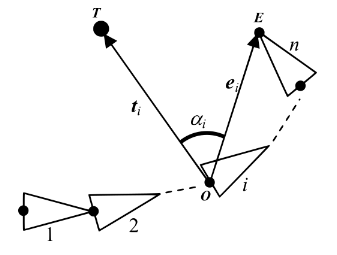
\includegraphics[width=0.9\textwidth,]{figures/background/CCD-geometry.png}
	\caption{CCD geometry}
	\label{fig:background/CCD geometry}
\end{figure}
\todo{make own figure}

\todo{experiments for runtime analysis in dependence of number of joints}
